%! Author = hugod
%! Date = 22/08/2023

% Preamble
\documentclass{iitFirstPage}

% Packages
\usepackage{amsmath}
\usepackage{amsfonts}
\usepackage{hyperref}
\usepackage{float}
\usepackage[acronym]{glossaries}
\usepackage{listings}
\usepackage{xcolor}
\usepackage[titletoc,title]{appendix}

% Graphics path
\graphicspath{{../resources/}}

% Initialization
\studentFirstName{Hugo}
\studentLastName{DABADIE}
\reportTitle{Vulnerabilities in Decentralized Applications}
\courseName{Research project}
\courseID{CS597}
\semester{January to August 2023}
\reportDate{September, 4th 2023}

% Setup
\hypersetup{
    colorlinks,
    citecolor=black,
    filecolor=black,
    linkcolor=black,
    urlcolor=black
}
\setglossarysection{subsection}
\definecolor{codegreen}{rgb}{0,0.6,0}
\definecolor{codegray}{rgb}{0.5,0.5,0.5}
\definecolor{codepurple}{rgb}{0.58,0,0.82}
\definecolor{backcolour}{rgb}{0.95,0.95,0.92}
\lstdefinestyle{mystyle}{
    backgroundcolor=\color{backcolour},
    commentstyle=\color{codegreen},
    keywordstyle=\color{magenta},
    numberstyle=\tiny\color{codegray},
    stringstyle=\color{codepurple},
    basicstyle=\ttfamily\footnotesize,
    breakatwhitespace=false,
    breaklines=true,
    captionpos=b,
    keepspaces=true,
    numbers=left,
    numbersep=5pt,
    showspaces=false,
    showstringspaces=false,
    showtabs=false,
    tabsize=2
}
\lstset{style=mystyle}

% Acronyms
\newacronym{dapp}{DApp}{Decentralized Application}
\newacronym{api}{API}{Application Programming Interface}
\newacronym{eip}{EIP}{Ethereum Improvment Proposals}
\newacronym{nft}{NFT}{Non-Fungible Token}

% Glossary
\makenoidxglossaries
\newglossaryentry{smartcontract}
{
    name={Smart Contract},
    description={Computer program that is stored and runs on a decentralized trustless network, such as a blockchain}
}

\newglossaryentry{dappdef}
{
    name={Decentralized Application},
    description={Application built on a decentralized network that consists of a smart contract backend and a user interface frontend}
}

\newglossaryentry{blockchain}
{
    name={Blockchain},
    description={Distributed database that maintains a continuously growing list of ordered records, called blocks}
}

\newglossaryentry{ethereum}
{
    name={Ethereum},
    description={Ethereum is the community-run technology powering the cryptocurrency ether and thousands of decentralized applications}
}

\newglossaryentry{replayattack}
{
    name={Replay Attack},
    description={Form of network attack in which valid data transmission is maliciously or fraudulently repeated or delayed}
}

\newglossaryentry{ecrecover}
{
    name={ecrecover},
    description={Function used to retreive the address used in a signature given the unsigned message}
}


% Document
\begin{document}

    \makeFirstPage

    \makeMargins


    \tableofcontents

    \newpage

    \listoffigures
    \begingroup
    \renewcommand{\clearpage}{\relax}
    \listoftables
    \endgroup

    \newpage

    \printnoidxglossaries

    \newpage


    \section*{Acknowledgments}

    I would like to express my sincere gratitude to the individuals who contributed to the successful completion of this report.

    First and foremost, I extend my deepest appreciation to Yue DUAN for his invaluable guidance, expertise, and mentorship throughout the research process.
    His insightful feedback and encouragement greatly enriched the quality of this work.

    $\\$

    I also extend my thanks to Sajad MEISAMI for his precious insights and contributions, which played a significant role in shaping the direction and depth of the study.
    His expertise and dedication have been instrumental in driving our research forward.

    $\\$

    Furthermore, my appreciation extends to Miguel OLEO BLANCO for his diligent efforts, insightful discussions, and collaborative spirit.
    His contributions added a unique perspective to the project and contributed to its overall excellence.

    I am genuinely grateful for the support and guidance I received from every team member, without whom this work would not have been possible.


    \section{Introduction}

    At the end of the engineer formation, the student, in France, has to do a 6-month internship called \textit{Projet de Fin d'Etudes} what stands for \textit{End of studies project}.
    Usually, an engineering student has already done another internship before this one.
    Ensimag encourages students to do at least one internship in the industry.

    $\\$

    The \textit{Projet de Fin d'Etudes} brings the university curriculum to a close, and is an opportunity for students to put into practice the skills acquired during their formation.
    It also develops their ability to work as part of a team, and prepares them to enter the professional world.

    $\\$

    I already have done two 3-month internships in the industry, and this is one of the reasons why I wanted to do this last internship in a research laboratory.
    I was drawn to cybersecurity, and I wanted to learn more about this field.
    This project applies cybersecurity to blockchain technology, which is a domain I had not studied during my formation.

    $\\$

    I was curious about discovering a new scope of computer science, especially because blockchain technologies are on-trend.
    Indeed, their decentralized nature, enhancing security, transparency, and efficiency in transactions makes them attractive.

    They enable smart contracts, tokenization, and innovations like decentralized finance and supply chain management.
    Despite challenges, blockchain's potential for disruption, investment opportunities, and real-world applications are driving its popularity.


    \section{Context}

    \subsection{Illinois Institute of Technology}

    Based in the global metropolis of Chicago, Illinois Tech is the only technology-focused university in the city.
    It offers degrees in engineering, science, architecture, business, design, human sciences, applied technology, and law.

    There are around 7,000 students at IIT of whom 3,000 are graduate students.
    62\% of the graduate students are international coming predominantly from India, China and Spain.

    There are several Master proposed by IIT.
    The Master of Computer Science degree program requires a core curriculum of three courses and seven other elective courses.
    One of these elective courses can be CS597: Research project.


    \subsection{CS597: Research project}

    This course counts as an elective course at IIT.
    The student is under the supervision of an IIT professor who gives him a project to work on.

    The goal is to be integrated in a research team, working for a project in a field that puts the student formation into practice.
    The length is variable and depends on the student and on the project.


    \subsection{Team}

    The team is under the supervision of Professor Yue DUAN.

    He is an assistant professor of computer science at Singapore Management University since this summer.
    Before this, he was a Gladwin Development Chair Assistant Professor at Illinois Institute of Technology.
    He had the postdoctoral training at Cornell University and University of Utah, and obtained his PhD in Computer Science from UC Riverside in 2019.

    His research interests mainly in different aspects of Computer Security, including mobile security, system security, software testing, blockchain security and AI security.

    $\\$

    Sajad MEISAMI is a PhD student at Illinois Institute of Technology since 2021, and he is responsible for this project.
    He has obtained a Master of Science from the Sharif University of Technology in 2020.

    $\\$

    The team is completed by two Master students.
    Miguel OLEO BLANCO who does a dual-degree Master at Illinois Institute of Technology, and with Universidad Pontificia Comillas.
    I am the last student of the team pursuing my dual-degree at Illinois Institute of Technology.


    \section{Motivations}

    Since the progress of Blockchain technology, a multitude of security challenges has arisen.
    These challenges commonly revolve around issues such as phishing attacks, scams, and flaws in the implementation of decentralized apps that operate on the blockchain.
    As a result, there is a growing necessity for users to ensure the security of these potentially harmful apps.
    The purpose of this project is to develop a tool capable of assessing the safety of apps by analyzing their source code, thereby aiding end users in making informed decisions.

    $\\$

    To accomplish this objective, a comprehensive investigation and research effort will be undertaken, focusing on the security landscape of decentralized applications and blockchain wallets.
    This will involve an exploration of the methods used in real-world \Glspl{dapp} and how they are integrated.
    Ultimately, the project aims to design and create a tool that can effectively carry out this analysis.
    
    $\\$

    Another motivation of this project is to reduce the scams and thefts that occur in \Glspl{dapp}, and in which millions of dollars are wasted every year for this reason.
    A clear example is one of the most recent thefts, in which 24 million euros in cryptocurrencies were instantly stolen.
    The goal is to develop a tool that can make the user more aware about the security of the applications that they are using.

    \section{Methodology}
    
    \subsection{Main objectives}

    The main purpose of the project is to give the end user of blockchain applications knowledge about the security of the application that he uses.
    To this end, one objective is the creation of a tool that will be able to determine the security level of the application and present it to the user.

    Another objective of this project is to generate a study on the security of the \Glspl{dapp} market with the information gathered from analyzing a large number of applications.
    This study will be presented in paper format to the scientific community after the defense of this work.

    Due to the research focus of this project, there are a number of objectives that have been generated while working towards the main objective.

    \subsection{Organization}

    \subsubsection{Spring semester}

    The project has begun with the spring semester, starting in early January and ending in May.
    During this period, I had three other courses, hence, I was not working full-time on the project.
    This organization is due to constraints with the dual-degree Master that I was pursuing.
    Indeed, I had to match the requirement from both IIT and Ensimag.

    Considering that particular situation, the work was given every week during a meeting.
    It was done during the week with the help from the other people on the project when needed.

    \subsubsection{Summer semester}

    Starting from May to August, during the summer semester, I was working full-time on the project.
    Daily meetings have been set up.
    The goal was to have a moment to exchange on the issues and the achievement made every day.

    However, the project was essentially done online because it was more convenient to meet.
    Indeed, during the project, there have been some familial issues and also some visa issues that prevent the team from meeting physically.
    Those unforeseen events have not affected the progress of the project.

    \section{Development}

    \subsection{Decentralized Applications}

    \subsubsection{Top 100 DApps}

    The work has begun with finding the most popular \Glspl{dapp}.
    We used the website Dapp Radar~\cite{dappradar}.
    It provides a list of different \Glspl{dapp} that can be sorted to get the most visited ones.
    We chose to sort the \Glspl{dapp} according to their traffic.

    It is important to get this list because they are more sensible as more people uses them.
    Moreover, some less popular \Glspl{dapp} try to impersonate the style of the most famous ones.
    Therefore, understanding the issues of the biggest ones can tell about the smallest.

    $\\$

    When we started the analysis, the most famous \Glspl{dapp} was Uniswap~\cite{uniswap}.
    The V3 and the V2 were in the top 10 \Glspl{dapp} (rank 1 and 8).
    Uniswap defines itself as an automated market maker.
    In practical terms, it is a collection of smart contracts that define a standard way to create liquidity pools, provide liquidity, and swap assets.
    The Uniswap Protocol is an open-source protocol for providing liquidity and trading tokens on Ethereum.
    It eliminates trusted intermediaries and unnecessary forms of rent extraction, allowing for safe, accessible, and efficient exchange activity.
    The protocol is non-upgradable and designed to be censorship resistant.
    The Uniswap Protocol and the Uniswap Interface were developed by Uniswap Labs.

    \subsubsection{Other DApps}

    Many more \Glspl{dapp} exists.
    One way to find a lot more of them is to make a search on GitHub.
    Indeed, the majority of \Glspl{dapp} are Open-source and their source code are available on this website.
    Using this method, we can easily find more than 58,000 GitHub repositories containing the keyword \textit{dapp} as the figure~\ref{fig:github-res} illustrates.

    \begin{figure}[H]
        \centering
        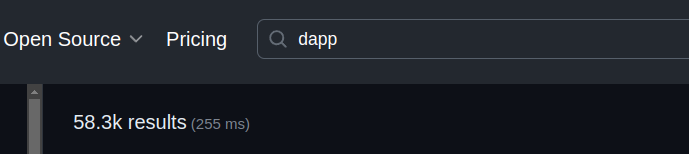
\includegraphics[width=0.79 \linewidth]{github/github-58k-results}
        \caption{GitHub results for dapp search}
        \label{fig:github-res}
    \end{figure}

    Finding more \Glspl{dapp} is essential for two main reasons.
    The first one is that if we only analyze the top 100 \Glspl{dapp}, we will miss a very high percentage of the existing \Glspl{dapp}.

    The other one is that usually, the more something is used, the more secure.
    Therefore, finding a vulnerability on a well-known \Gls{dapp} seems to be more difficult.
    Furthermore, a vulnerability on a less popular \Gls{dapp} can still lead to huge damage.

    \subsection{Analysis of programming languages used}

    \begin{table}[H]
        \begin{center}
            \begin{tabular}{|c|c|}
                \hline
                \textbf{Programming Language}   & \textbf{Number of \Glspl{dapp}}\\
                \hline
                \hline
                TypeScript   & 52                        \\
                \hline
                JavaScript    & 29                          \\
                \hline
                Unknown & 15                              \\
                \hline
                Python & 3                                \\
                \hline
                Cadence & 1                               \\
                \hline
            \end{tabular}
        \end{center}
        \caption{Different programming languages used by top 100 \Glspl{dapp}}
        \label{tab:program-lang}
    \end{table}

    The table~\ref{tab:program-lang} shows the different languages mainly used to develop the top 100 \Glspl{dapp}.
    More than a half are written using TypeScript and a third are written with JavaScript.
    As TypeScript and JavaScript are really similar languages, the analysis will focus on this two languages.
    It represents a large majority of the most popular \Glspl{dapp}.

    15 \Glspl{dapp} have an unknown programming language because it was not possible to find their source code.
    Finally, only 4 of the top 100 \Glspl{dapp} are not written in JavaScript or TypeScript for sure.
    This is why our analysis does not include \Gls{dapp} not written in JavaScript or TypeScript.

    \subsection{Blockchain}
    
    \subsubsection{What is a blockchain?}

    A \Gls{dapp} is an application based on a \gls{blockchain} which can be described as a list of blocks (chain of blocks).
    These blocks are linked with cryptographic methods.
    Each one has the hash, which represents the data of a block, of the previous block.
    It also contains a timestamp and the information of a transaction that had been made.

    A blockchain is a digital ledger that operates in a decentralized and distributed manner, accessible to the public.
    It's designed to record transactions across multiple computers in a way that prevents retroactive changes without modifying all subsequent blocks and gaining agreement from the network.
    
    A blockchain may be used, for instance, to process payment, to monitor supply chains, to share data, for copyright and royalties protection.

    \subsubsection{Wallet on a blockchain}

    One of the most common application of \gls{blockchain} is the management of cryptocurrency wallet.
    The most used wallet is MetaMask, another well-known one is Binance.
    The goal of these applications is to enable users to store cryptocurrency and transfer them.
    It provides an interface to interact with the blockchain.

    \clearpage

    MetaMask is a browser plugin that acts as an \Gls{ethereum} wallet, and easy to use as the figure~\ref{fig:meta-extension} depicts.
    By connecting to MetaMask to Ethereum-based \Glspl{dapp}, users can spend their coins in games, stake tokens in gambling applications, and trade them on decentralized exchanges (DEXs).
    It also provides users with an entry point into the emerging world of decentralized finance.

    \begin{figure}[H]
        \centering
        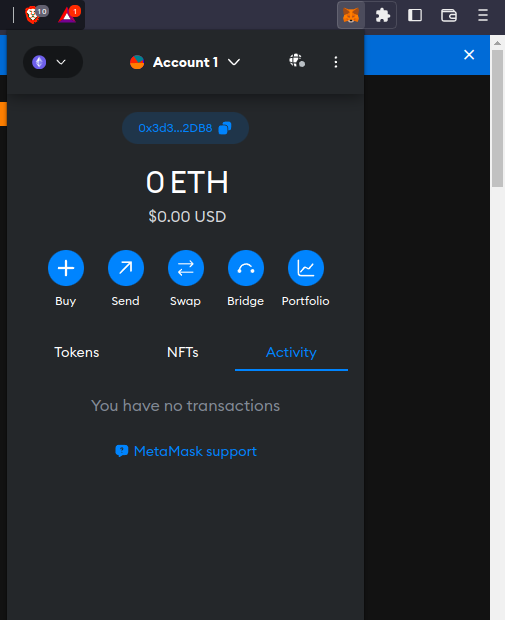
\includegraphics[width=0.49 \linewidth]{metamask/metamask_extension}
        \caption{Metamask extension}
        \label{fig:meta-extension}
    \end{figure}

    MetaMask provides an \Gls{api} to integrate their wallet onto other \Glspl{dapp}.


    \subsection{API used in DApps}

    \subsubsection{MetaMask API}

    The first step was to analyze the MetaMask \Gls{api} in order to determine the most sensible ones.
    The analysis is based on the official MetaMask documentation~\cite{metamaskdoc} and on the MetaMask API playground~\cite{metamaskplayground}.

    $\\$

    As for the first documentation, it is very scarce, since it only collects some very select methods.
    Among these methods are the restricted methods, which are the methods that require permissions.
    Because of this, the methods in this documentation are very limited, and many are not well-developed.

    \clearpage

    Besides, the Metamask test page contains almost all available methods.
    This page also briefly explains the functionality of the methods, structure of the input and response parameters.
    Moreover, it also describes which of them are mandatory and which are optional.
    However, since it is not the official documentation webpage, it may not be up-to-date, and the results must be double checked.

    $\\$

    The analysis has been made using a spreadsheet to gather the results as the figure~\ref{fig:meta-api-gsheet} illustrates.
    It includes the different parameters used by the \Glspl{api} with the distinction of mandatory and optional parameters.
    Then, the next column, \textit{Permission / Confirmation} indicates whether the \Gls{api} requires a user confirmation via a pop-up or not.
    This column has some more details in another column.
    The column \textit{Return} shows the type of the object returned by the \Gls{api}.

    $\\$

    Finally, the column \textit{Differences} explains what is different from the MetaMask documentation to the \Gls{eip} corresponding to this \gls{api}.
    The \Glspl{eip} are the standards for blockchain interaction \gls{api} and will be discussed later.


    \begin{figure}[H]
        \centering
        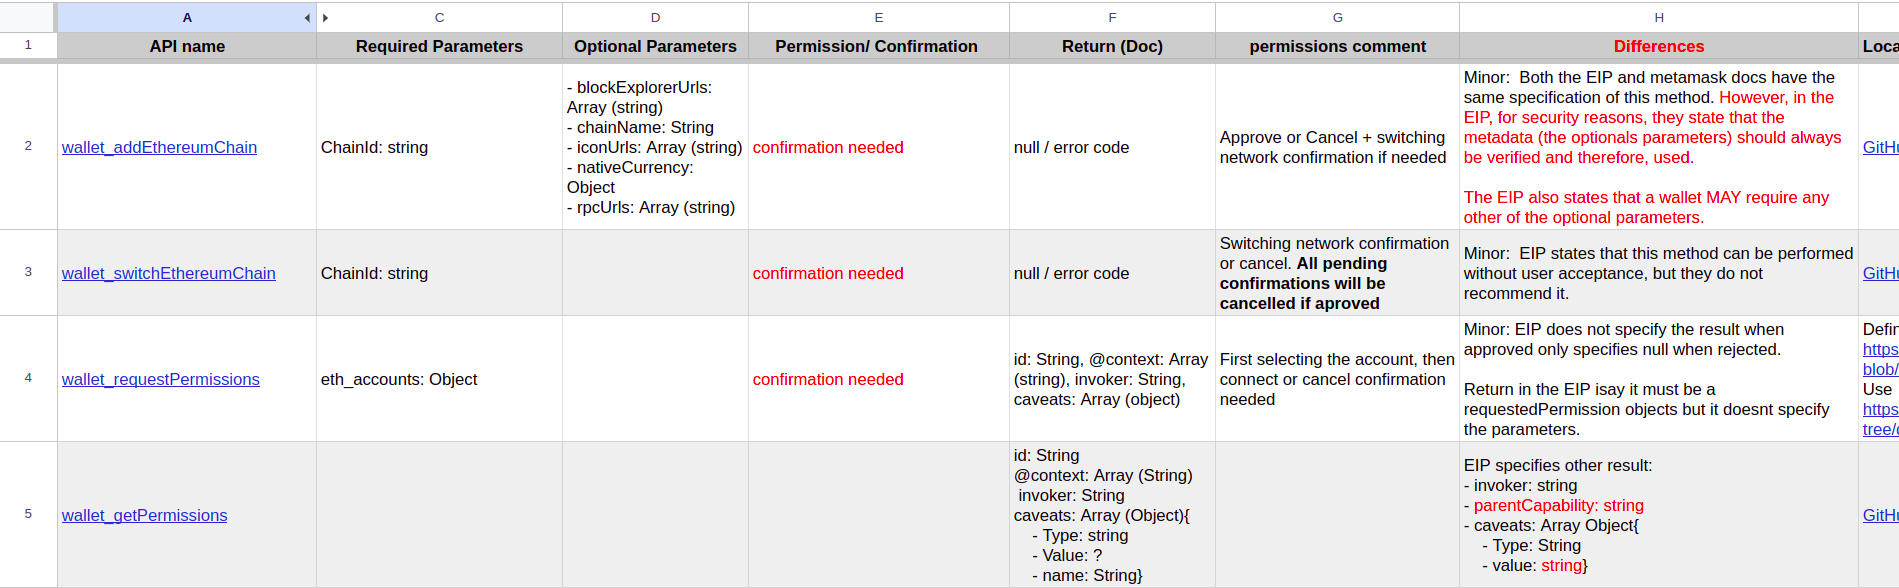
\includegraphics[width=0.99 \linewidth]{metamask/metamask_api_gsheet}
        \caption{Metamask API analysis}
        \label{fig:meta-api-gsheet}
    \end{figure}

    $\\$

    \subsubsection{Ethers.js and Web3.js API}

    Ethers.js provides also many \Glspl{api} to interact with the Ethereum Blockchain and its ecosystem.
    It was originally designed for usage with ethers.io and has since expanded into a more general-purpose library.
    The Ethers.js documentation~\cite{ethersdoc} is more complete than the MetaMask documentation~\cite{metamaskdoc} what simplifies the analysis.

    $\\$

    Web3.js is the other major \Glspl{api} provider to interact with the blockchain.
    It identifies as a collection of libraries that allow the user to interact with a local or remote ethereum node.
    As for Ether.js, the Web3.js documentation~\cite{web3doc} is also very complete and provides information for every method that is possible to use.

    \clearpage

    In this project, we have not studied the security of these two libraries, and we chose to focus our work on the Metamask \Gls{api}.
    Since it is possible to link the MetaMask portfolio with applications developed with Ether.js and Web3.js, by studying MetaMask, we also studied the latter two libraries.
    Because of this, the documentation has been made method by method, as for MetaMask, with mandatory parameters, optional parameters, method return, etc.

    The most important thing is to document the methods that correspond to those of Metamask.
    Therefore, in the spreadsheet, three sheets have been created (one for Metamask, one for Ether.js and one for Web3.js), and the column numbers match the methods.
    That is, the method of Metamask in one particular row, corresponds to the same methods, but from EtherJS and from Web3JS in the same row.


    \subsection{EIP}

    \subsubsection{General concept}

    \Glspl{eip}, which stands for Ethereum Improvement Proposals~\cite{eipdef}, play a crucial role in the evolution of the Ethereum blockchain.
    They are essentially sets of guidelines that propose and describe potential enhancements, additions, or changes to the Ethereum network's functionality.
    These proposals can cover a wide range of topics, such as introducing new features, improving existing processes, or suggesting updates to the overall architecture.

    Each \Gls{eip} is like a detailed blueprint, providing technical specifications and documentation for the proposed alteration.
    This documentation is essential for the Ethereum community to understand the scope, purpose, and implementation details of the suggested change.
    \Glspl{eip} is similar to a source of truth, serving as the authoritative reference point for anyone who wishes to comprehend the intricacies of a particular proposed improvement.

    $\\$

    One of the significant aspects of the \Gls{eip} process is its decentralized nature.
    It encourages collaboration and input from various stakeholders in the Ethereum ecosystem.
    Developers, researchers, users, and other community members can engage in discussions, provide feedback, and contribute their expertise to refine and validate the proposal.
    This collaborative effort helps ensure that proposed changes are well-vetted and aligned with the broader Ethereum community's goals and values.

    The \Gls{eip} process also serves as the foundation for discussing and implementing network upgrades.
    When a proposal gains significant consensus and is thoroughly reviewed, it can become part of a network upgrade, often referred to as a hard fork.
    These upgrades can introduce substantial changes to the Ethereum protocol, enhancing its capabilities, performance, and security.

    \clearpage

    Furthermore, \Glspl{eip} provide a framework for establishing application standards within the Ethereum ecosystem.
    By proposing standardized processes or conventions, \Glspl{eip} contribute to a more cohesive and interoperable environment for \Glspl{dapp} and \glspl{smartcontract}.
    This standardized approach simplifies development and enhances the overall user experience by ensuring consistency across various applications built on Ethereum.

    In essence, \Glspl{eip} are the backbone of Ethereum's continuous evolution.
    They embody the collaborative spirit of the Ethereum community, ensuring that proposed improvements are thoroughly examined, technically sound, and aligned with the platform's overarching vision of a decentralized and innovative blockchain ecosystem.

    \subsubsection{EIP721}

    The EIP721~\cite{eip721} introduces a standardized \Gls{api} that enables the integration of \Glspl{nft} into \glspl{smartcontract}.
    This established standard furnishes fundamental functionality for monitoring and facilitating the transfer of \Glspl{nft}.

    $\\$

    This \Gls{eip} is inspired by the ERC-20 token standard, defined in the EIP20~\cite{eip20}.
    The introduction of the ERC-721 standard (EIP721) was necessary because the ERC-20 standard (EIP20) was not suitable for representing non-fungible assets.
    Fungible tokens are essentially identical and can be exchanged on a one-to-one basis, making them ideal for representing divisible assets like currencies.
    However, non-fungible assets are fundamentally distinct and unique, and they required a different standard to accurately represent their ownership, attributes, and individuality.

    $\\$

    EIP721 addressed this need by providing a standardized way to create and manage non-fungible tokens, allowing developers to accurately represent ownership of unique assets in a consistent manner.
    This has opened the door to a wide range of applications such as digital art marketplaces, virtual collectibles, decentralized games, and more, where the uniqueness and individual characteristics of each asset are essential.

    \subsubsection{EIP712}

    The EIP712~\cite{eip712} defines standards that allow developers to specify the structure of data in a way recognizable by both humans and machines.
    This structured data can include various fields and types of information, and it's often used to represent specific interactions, transactions, or messages that need to be signed by users.

    One of the key benefits of EIP712 is that it helps prevent certain types of attacks, like \gls{replayattack}, which will be discussed later, by ensuring that the signed data includes contextual information that uniquely identifies the transaction.
    This makes it harder for attackers to reuse signed data in different contexts.

    $\\$

    The link between EIP721 and EIP712 comes into play when dealing with \Glspl{nft} created according to the ERC-721 standard.
    Since \Glspl{nft} represent unique and often valuable assets, their transactions need to be securely authorized and verified.

    EIP712 is commonly used in the context of \Glspl{nft} to define and structure the data associated with token-related actions, such as transferring ownership of an \Gls{nft} from one address to another.
    By structuring this data using the EIP712 format, it becomes easier to generate and verify digital signatures that prove the authenticity and authorization of transactions involving \Glspl{nft}.

    $\\$

    In essence, EIP712 enhances the security and trustworthiness of interactions involving \Glspl{nft} (such as transfers) by providing a standardized way to structure and sign data, which can be essential in preventing unauthorized or malicious activities.

    \clearpage

    \subsection{Signing methods in MetaMask}
    
    \subsubsection{Importance of signing methods}

    In the blockchain, the implementation of different signature methods is necessary.
    All information that needs to be transmitted through this blockchain is signed for the security and integrity of the data, and to confirm that the sender is the expected one.
    Over the years, new and more secure forms of signatures have been discovered.
    Metamask has implemented different signature methods over time.

    $\\$

    While signing methods and wallet applications like MetaMask are designed to enhance security and user control in the world of blockchain and cryptocurrencies, they can also introduce vulnerabilities if not used or implemented correctly.
    This is the reason why the project focuses on signing methods provided by MetaMask.
    Their implementation in \Glspl{dapp} is a crucial point of security.


    \subsubsection{eth\_sign}

    The first method that had been implemented by MetaMask is the least secure.
    Indeed, in the popup presented to the user when confirming the signature, the message is not readable, as the figure~\ref{fig:eth-sign-message} shows.

    \begin{figure}[H]
        \centering
        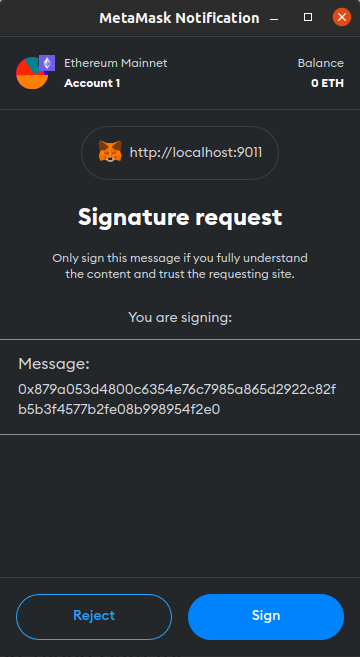
\includegraphics[width=0.39 \linewidth]{signature/eth_sign_message}
        \caption{eth\_sign pop-up message}
        \label{fig:eth-sign-message}
    \end{figure}

    Therefore, many attacks were based on presenting the user with this signature.
    As it is not readable, they sign it thinking that it is a legitimate transaction, whereas the application makes them sign something else.
    As can be seen in the following image, the message to be signed is a hexadecimal string that arises from hashing the signature, so the user cannot understand it.

    $\\$

    When this study was initiated, this method was not recommended.
    Now, Metamask itself has listed this signature method as deprecated and prevents user from using it.
    As the figure~\ref{fig:eth-sign-warning} illustrates, the user who wants to sign a message with this \Gls{api} needs to activate it in MetaMask advanced settings.
    They also have had a warning to make sure people are aware of the risk of this signing method.

    \begin{figure}[H]
        \centering
        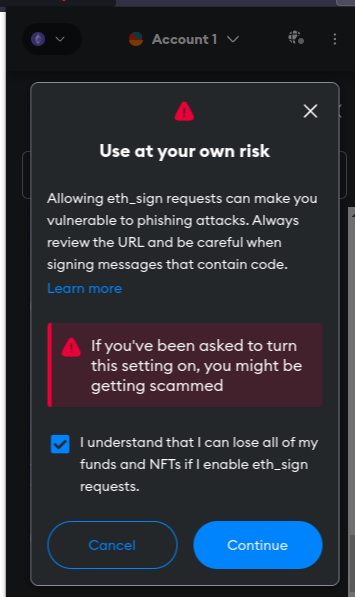
\includegraphics[width=0.49 \linewidth]{signature/eth_sign_warning}
        \caption{eth\_sign warning message when trying to enable this \Gls{api}}
        \label{fig:eth-sign-warning}
    \end{figure}

    In general, applications already use the other more modern methods, so the application will work without any problem.
    However, many \Glspl{dapp} still use the \textit{eth\_sign} method as a signature method what breaks some functionalities of those websites.

    \clearpage

    \subsubsection{personal\_sign}

    The \textit{personal\_sign} method was introduced by Metamask to fix the signature message not being readable.
    This function is the easiest way to implement this.
    The main problem with this method, since the message is readable, is that it makes it less efficient to be processed in the blockchain as the message can be quite long.
    This specific method is not very efficient.
    Even so, many applications still use this method because it is basic.
    The figure~\ref{fig:personal-sign-message} shows the appearance of the message presented to the user when executing this method.

    \begin{figure}[H]
        \centering
        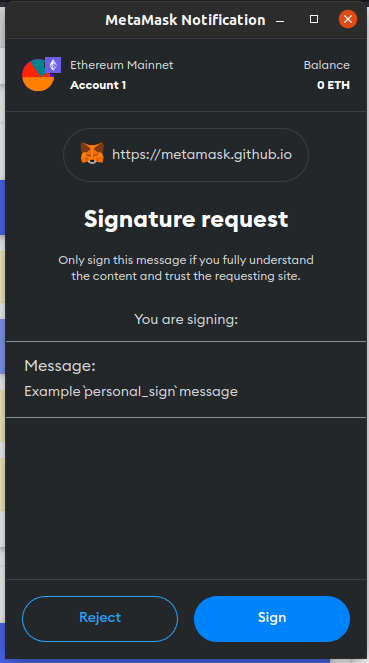
\includegraphics[width=0.49 \linewidth]{signature/personal_sign_message}
        \caption{personal\_sign pop-up message}
        \label{fig:personal-sign-message}
    \end{figure}

    \clearpage

    \subsubsection{eth\_signTypedData}

    The method \textit{eth\_signTypedData} was introduced by EIP712.
    The EIP712 specification changed several times, resulting in multiple versions of \textit{eth\_signTypedData}.

    As the figure~\ref{fig:signtypeddata-sign-message} shows, the pop-up message of \textit{eth\_signTypedData} represents structured data what makes it more human readable.
    Moreover, being structured data makes it easy to compute for the blockchain as it can be encoded efficiently.
    It also cannot impersonate Ethereum transactions.

    \begin{figure}[H]
        \centering
        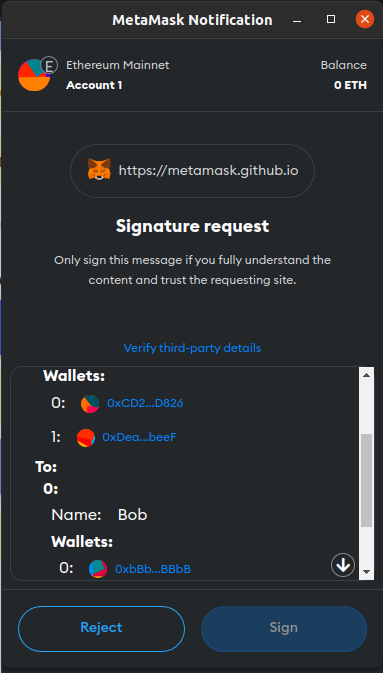
\includegraphics[width=0.45 \linewidth]{signature/eth_signtypeddatav4_message}
        \caption{eth\_signTypedDataV4 pop-up message}
        \label{fig:signtypeddata-sign-message}
    \end{figure}

    The first version of this \Gls{api} (\textit{eth\_signTypedData\_v1} or \textit{eth\_signTypedData}) was subject to some attacks, such as \glspl{replayattack}.
    Version 3 introduced some mechanisms to prevent from those attacks, like the field domain inside the message to sign (more precision will be given later).
    Finally, the last and only version recommended to use by MetaMask is the v4, which includes full support of arrays and recursive data structures.
    The missing v2 represents an intermediary design that the Cipher browser implemented.

    $\\$

    We chose to focus on \textit{eth\_signTypedData} because \textit{eth\_sign} is already deprecated and not recommended.
    Furthermore, as \textit{personal\_sign} is not very efficient and \textit{eth\_signTypedData} is more complex, our analysis focuses on this \gls{api}.

    \clearpage

    \subsection{Operation of eth\_signTypedData}

    \subsubsection{Method arguments defined in EIP712}

    EIP712 defines several measures to enhance the security of signing methods.
    The one that interests us the most is the inclusion of a field named \textit{domainSeparator}.
    This field includes four or five items, because the last is optional, variable:

    \begin{itemize}
        \item name: the user-readable name of signing domain, usually the name of the \Gls{dapp}.
        \item version: the current major version of the signing domain.
        \item chainId: the user-agent should refuse signing if it does not match the currently active chain.
        \item verifyingContract: the address of the contract that will verify the signature.
        \item salt (optional): a disambiguating salt for the protocol.
    \end{itemize}

    The purpose of these fields is to make the signature linked with the \Gls{dapp}.
    Before, the same message signed by the same person on different \Glspl{dapp} had the same signature.
    Now, with, for instance the name of the \Gls{dapp}, the signature differs on two different \Glspl{dapp} even if the message signed is the same.

    $\\$

    The purpose of \textit{chainId} is to differentiate different blockchain of the same \Gls{dapp}.
    Indeed, some huge \Gls{dapp} uses several blockchain.
    The value of \textit{verifyingContract} prevents an attacker from using a malicious contract to verify the signature.

    $\\$

    \subsubsection{Creation of a test Dapp}

    To analyze more precisely how this method was working, the best solution is to implement a \Gls{dapp}.
    This allows trying every possibility for the argument which can be given to the method.
    This step is crucial because the MetaMask documentation is not precise enough and does not indicate which field can be omitted or not.

    $\\$

    Determining which field is mandatory and which one is not plays a pivotal role in the analysis.
    Indeed, the majority of the fields required by \textit{eth\_signTypedData} plays a role in the security of the signing method.
    Therefore, if malicious \Glspl{dapp} are able to omit some verification field, it can lead to unsafe behaviour.

    \begin{figure}[H]
        \centering
        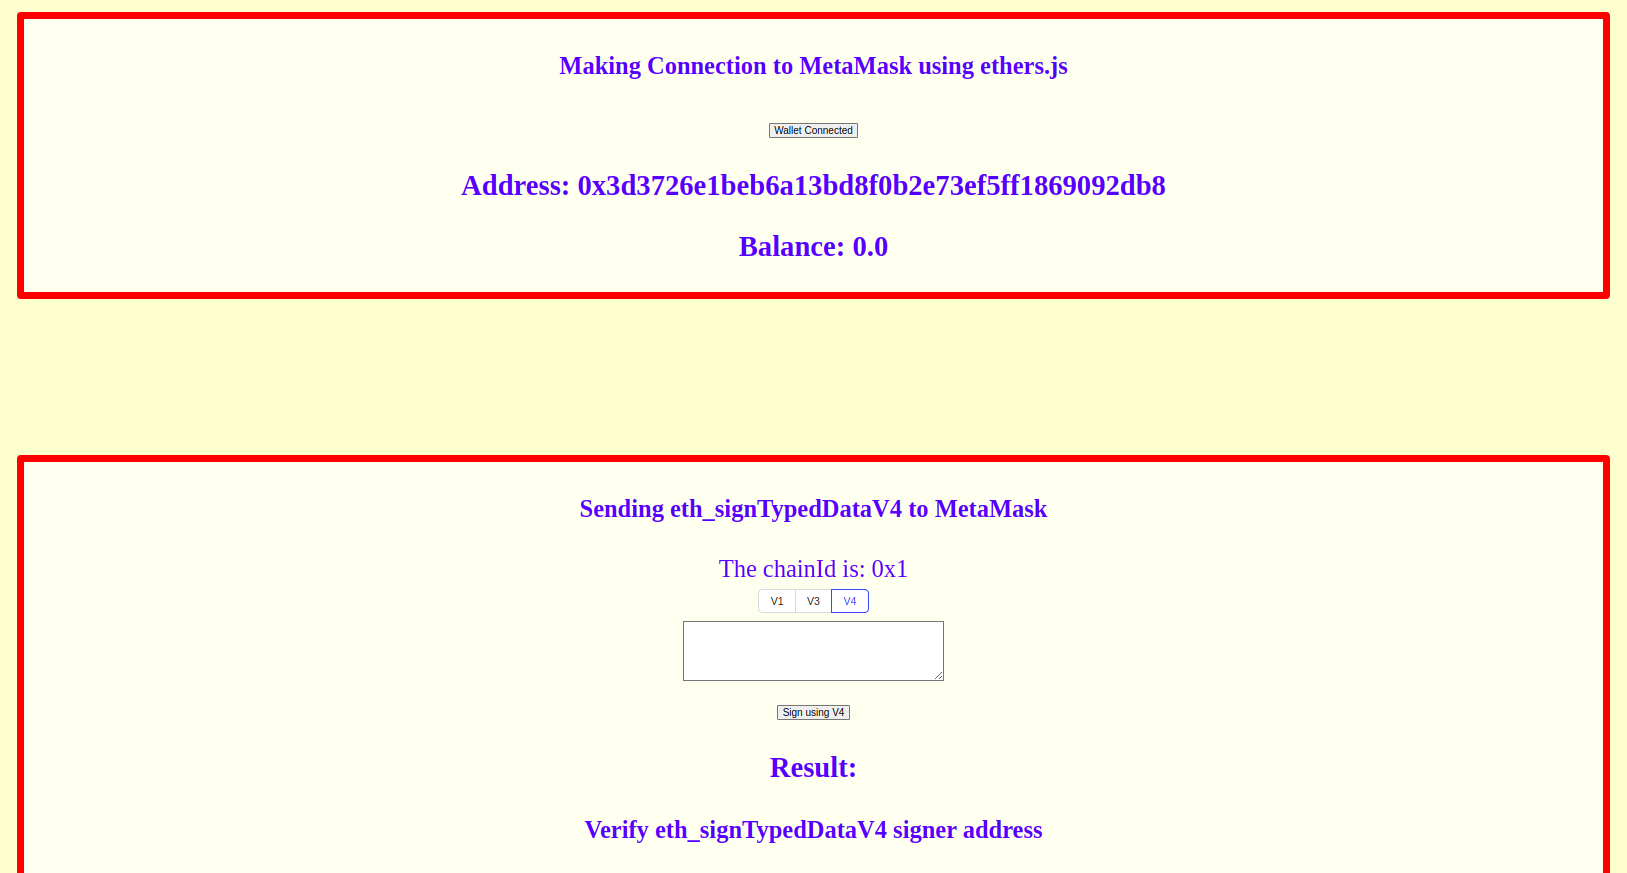
\includegraphics[width=0.9 \linewidth]{metamask/dapp_test_hugo}
        \caption{DApp created to test eth\_signTypedData}
        \label{fig:test-dapp}
    \end{figure}

    The figure~\ref{fig:test-dapp} is a picture of the \Gls{dapp} created that has enabled us to understand how MetaMask handles arguments.
    We can try to sign a message with different structured message and then analyze the answer.

    \subsubsection{Mandatory fields}

    The figure~\ref{fig:payload-signtypeddata} shows an example of a payload as defined by the EIP712.

    $\\$

    There are four mandatory sections:

    \begin{itemize}
        \item domain: this is the \textit{domainSeparator} that we discussed earlier.
        \item message: this field represents the useful data that we want to transfer.
        \item types: this defines the types of the different fields present inside the payload.
        \item primaryType: this gives information about the message sent.
    \end{itemize}


    \begin{figure}[H]
        \centering
        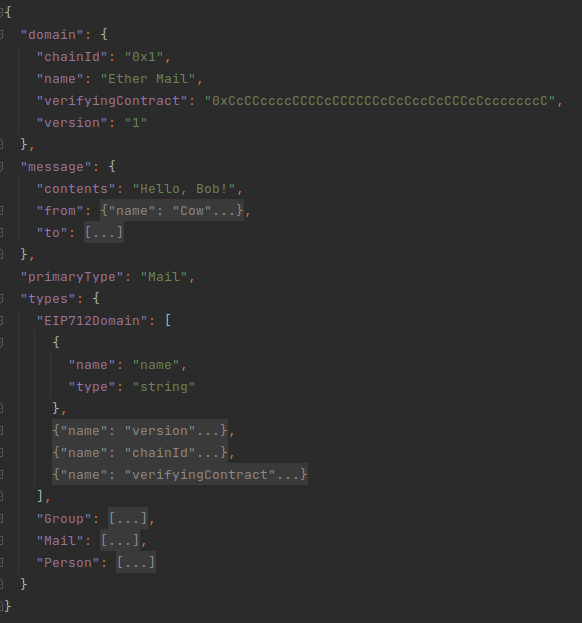
\includegraphics[width=0.69 \linewidth]{signature/payload_signtypeddata}
        \caption{Example of message sent using eth\_signTypedData}
        \label{fig:payload-signtypeddata}
    \end{figure}


    The analysis has highlighted some constraint about those fields.
    First, every field included in the payload must be defined in \textit{types}.
    Otherwise, MetaMask would ignore the missing field.

    Then, \textit{primaryType} must match a type defined in \textit{types}.
    MetaMask gives an error if this condition is not met.

    The \textit{message} and \textit{domain}  fields only need to contain every field declared in \textit{types}.

    $\\$

    This means that only the four sections are mandatory but can be empty, except for \textit{primaryType} and \textit{types} which need at least one value.
    Nonetheless, \textit{domain} may be an empty string and MetaMask will accept the payload.
    Due to this, the \Gls{dapp} that uses \textit{eth\_signTypedData} is able to make the user sign a message without \textit{domainSeparator}.
    Nevertheless, we explained earlier that \textit{domainSeparator} prevents from different attacks, hence, this particular point is a vulnerability in \textit{eth\_signTypedData}.

    \clearpage

    \subsection{Analysis of signing methods in DApps}

    \subsubsection{Finding every usage of signing methods}

    After finding a vulnerability in \textit{eth\_signTypedData}, the next step is to find which \Glspl{dapp} uses this method.
    Moreover, we also want to find the usage of the other signing methods.
    Therefore, a bash script, available in the appendix~\ref{sec:find-signing-methods-script}, has been developed.

    $\\$

    The principle of the script is to download every GitHub repository from a list, and then search within every file for a particular string.
    In our case, we want to search for \textit{eth\_sign}, \textit{personal\_sign} and signTypedData (not \textit{eth\_signTypedData}, because sometimes it shadows some interesting match).
    Once we find the string, we write in an output file, the line and file corresponding to the matching string.

    $\\$

    Then, thanks to other bash and python scripts, the results are formatted to a csv file which is easy to import in a spreadsheet to make the results more human-readable.
    The figure~\ref{fig:dapp-sign-result} shows the spreadsheet in which the results are stored.

    \begin{figure}[H]
        \centering
        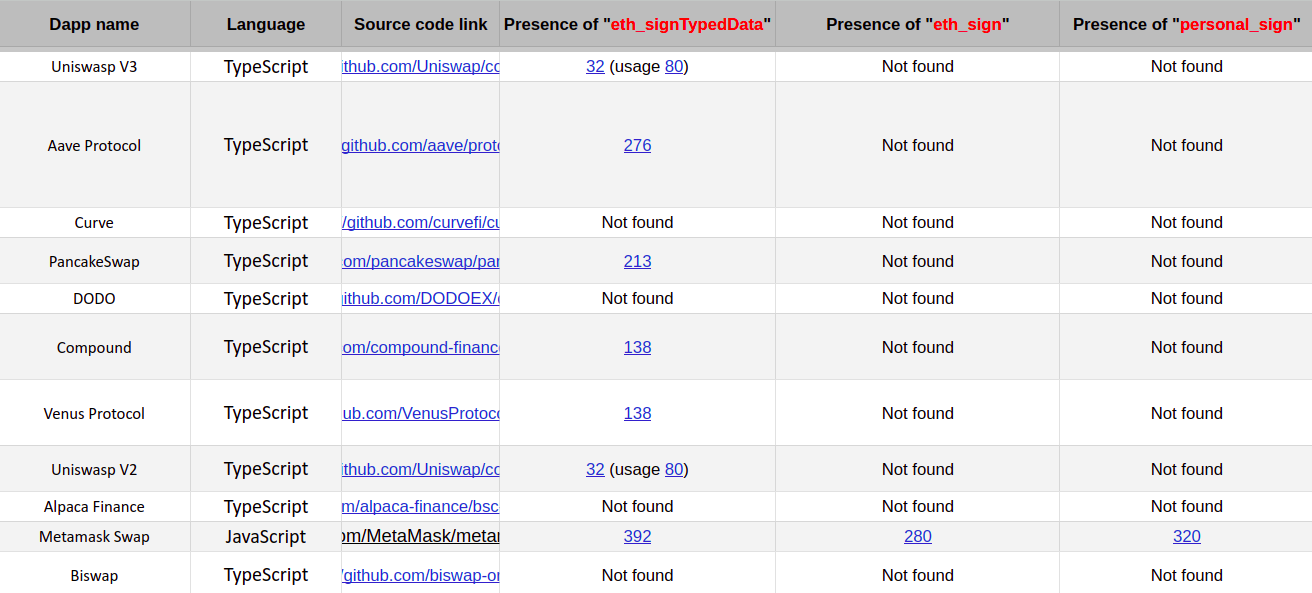
\includegraphics[width=0.9 \linewidth]{signature/dapp_signature_result}
        \caption{Spreadsheet which stores the results of signing methods usage in DApps}
        \label{fig:dapp-sign-result}
    \end{figure}

    \subsubsection{Collecting more DApps}

    Analyzing the top 100 \Glspl{dapp}, gives a good overview of signature methods usage.
    However, as mentioned earlier, we cannot limit the analysis to those \Glspl{dapp}.
    Therefore, it is necessary to find a way to collect more applications.
    
    $\\$
    
    GitHub gives an \Gls{api}~\cite{githubapi} that allows getting the results of a search.
    Using the \Gls{api} makes possible to develop a script to automate the finding of new \Glspl{dapp}.

    However, GitHub limits to 100 repositories that can be found by call to the \Gls{api}.
    The solution found is to get the first 100 results, and then get the next 100 until there is no more result available.

    \clearpage

    This has highlighted another limitation to GitHub \Gls{api}.
    Indeed, only the first 1000 results can be accessed no matter the filter we use.
    Nonetheless, this script has enabled to collect more than 2,000 other \Glspl{dapp}, using different queries.
    Then, the duplicate repositories are eliminated with another bash script.

    Those scripts have enabled to make the analysis a lot more solid and thorough.

    $\\$

    The figure~\ref{fig:githubsearchrepo} shows the main part of the bash script that calls the GitHub \Gls{api}.
    Using the filter \textit{per\_page}, it is possible to select different range of 100 repositories.

    \begin{figure}[H]
        \centering
        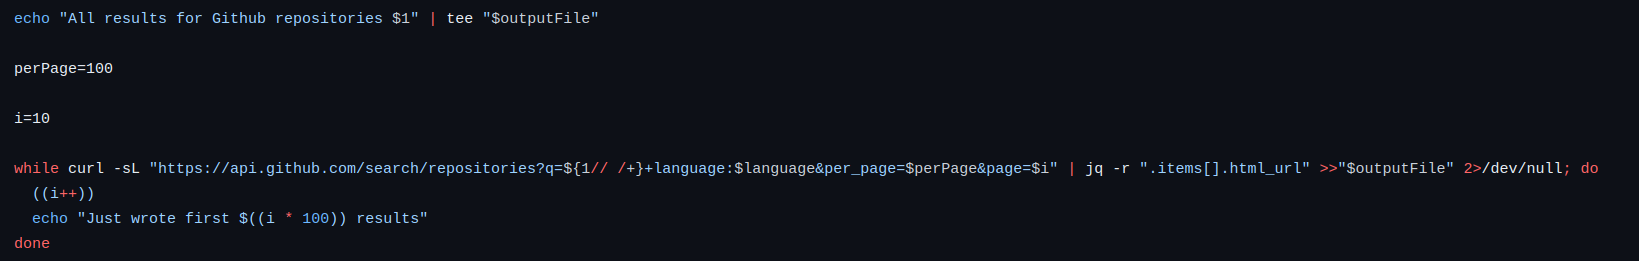
\includegraphics[width=0.99 \linewidth]{github/github_search_repo}
        \caption{Bash script to collect GitHub repositories from a query}
        \label{fig:githubsearchrepo}
    \end{figure}

    \subsubsection{Usage of signing methods}

    We have implemented a bash script, available in appendix~\ref{sec:combine-all-scripts}, that combines all the different other scripts mentioned above.
    This script enables to automate the analysis of \Glspl{dapp} source code to find every usage of signing methods.
    It also formats the result to a csv file, making the results easy to read in a spreadsheet.

    $\\$

    After running the scripts, we obtained the results presented in table~\ref{tab:res-signing-analysis}.

    \begin{table}[H]
        \begin{center}
            \begin{tabular}{|c||c|c|}
                \hline
                \textbf{Signing method}   & \textbf{Top 100 \Glspl{dapp}} & \textbf{On 2,490 \Glspl{dapp}}\\
                \hline
                \hline
                \textit{eth\_signTypedData}   & 37\%    & 5\%              \\
                \hline
                \textit{eth\_sign}    & 19\%       & 14\%     \\
                \hline
                \textit{personal\_sign} & 13\%       & 10\%              \\
                \hline
            \end{tabular}
        \end{center}
        \caption{Analysis of usage of signing methods in \Glspl{dapp}}
        \label{tab:res-signing-analysis}
    \end{table}

    The results of the analysis highlight several points.
    The first one is that signing methods are more used in top 100 \Glspl{dapp}.
    It can be explained because the most visited \Glspl{dapp} are usually the ones with more functionalities, and smaller website can delegate the signing part to other applications.

    The analysis also shines a light on the fact that \textit{eth\_sign} is still a lot used by \Glspl{dapp} even the biggest ones (the $10^{th}$ one has been using this method).

    $\\$

    These results also spotlight that on less visited \Glspl{dapp} \textit{eth\_sign} is even more used than on the top 100.
    The figure~\ref{fig:repartition-top100} and the figure~\ref{fig:repartition-all}, which present the repartition of signing methods usage on both scopes of the analysis, allows to emphasize this point.


    \begin{figure}[H]
        \centering
        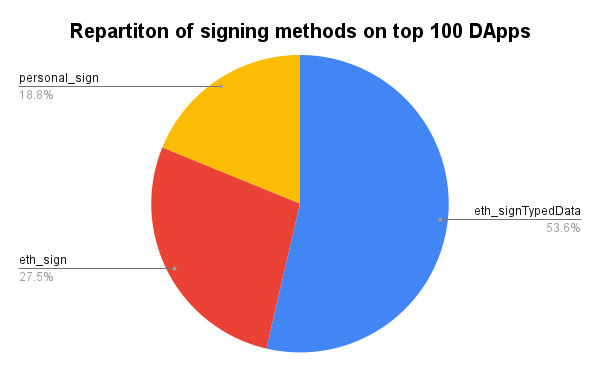
\includegraphics[width=0.69 \linewidth]{signature/repartiton_top100_dapps}
        \caption{Repartition of signing methods on top 100 \Glspl{dapp}}
        \label{fig:repartition-top100}
    \end{figure}

    \begin{figure}[H]
        \centering
        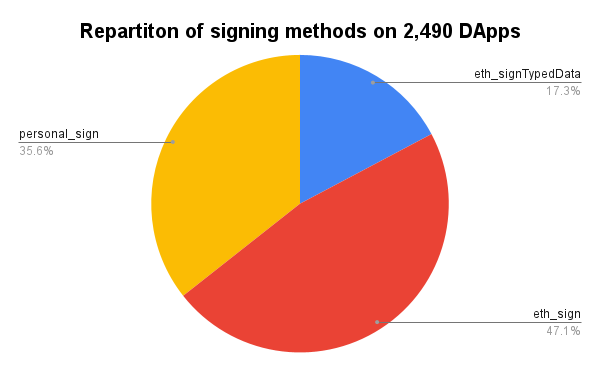
\includegraphics[width=0.69 \linewidth]{signature/repartiton_all_dapps}
        \caption{Repartition of signing methods on 2,490 \Glspl{dapp}}
        \label{fig:repartition-all}
    \end{figure}

    Indeed, the two figures~\ref{fig:repartition-top100}~and~\ref{fig:repartition-all} point out the fall in the usage of the safer \textit{eth\_signTypedData} in favor to the unsecure \textit{eth\_sign}.
    More than half of signing methods used in top100 are \textit{eth\_signTypedData} whereas, in all \Glspl{dapp} of the analysis, it is only around a sixth.
    Moreover, the usage of \textit{eth\_sign} increases from 27.5\% to 47.1\%.
    The high usage of this unsafe method reveals a vulnerability in the construction of many \Glspl{dapp}.

    \clearpage

    \subsection{Smart contracts implementation}
    
    \subsubsection{Smart contracts role}

    The goal of \glspl{smartcontract} is to execute code on the blockchain.
    What we are interested in is the verifications of signature that are made online.
    As a matter of fact, every \Gls{dapp} needs to verify that the user who wants to make a sensible action, for instance, transferring funds.
    The application makes this verification on \glspl{smartcontract} deployed online.
    The specification of the implementation is, among others, described in EIP721.

    $\\$

    \subsubsection{ecrecover}

    The \textit{\gls{ecrecover}} function is a crucial element found within Ethereum smart contracts, primarily serving the purpose of signature verification for messages.
    When invoked, it requires specific input parameters to operate effectively: the hash of the message being verified and the signature's individual components, namely \textit{v}, \textit{r}, and \textit{s}.

    By employing intricate elliptic curve calculations, this function is capable of recovering two distinct potential public keys from the provided signature.
    The recovery process is facilitated by the recovery id \textit{v}, which aids in pinpointing the accurate public key.

    $\\$

    Subsequently, the Ethereum address affiliated with the signer of the message is generated through a process involving hashing the computed public key.
    The crux of this process revolves around confirming whether the generated address aligns with the expected address of the signer.

    In practical terms, this cryptographic mechanism finds extensive application in enabling authentication and authorization protocols within smart contracts.

    $\\$

    The proper implementation of \textit{\gls{ecrecover}} into \glspl{smartcontract} plays a pivotal role in upholding the security and integrity of the entire system.
    Essentially, the overarching purpose of this function lies in its ability to fortify \glspl{smartcontract} against fraudulent actions by effectively validating digital signatures.

    $\\$

    \subsubsection{Nonce and deadline}

    As considered with the description of EIP712 above, \textit{domainSeparator} is a crucial point of the signature security.
    It helps to ensure that the signature is from the right \Gls{dapp}.
    However, it does not prevent from \glspl{replayattack}.

    Indeed, if an attacker steals a signature that gives the permission to withdraw a certain amount of money, he can validate the transaction many times.
    This entails a huge loss of money for the victim.

    $\\$

    The first mechanism that \Glspl{dapp} have introduced is \textit{deadline}.
    It is a timestamp included in the signature making the signature to be expired after a certain date.
    This is often used for voting \Glspl{dapp}, because it prevents people from voting after the end of the election.

    $\\$

    The last tool used is \textit{nonce}.
    A \textit{nonce} stands for \textit{number used once} in the realm of blockchain and cryptography.
    It prevents double spending by requiring each transaction to have an unique \textit{nonce}.
    In \Gls{ethereum} and \glspl{smartcontract} platforms, \textit{nonces} establish transaction order and prevent \glspl{replayattack}.
    In essence, \textit{nonces} bolster security and ensure orderly processes in blockchain operations.

    \subsection{Classification of DApps}

    \subsubsection{Purpose of classification}

    The next step is to analyze the \glspl{smartcontract} of the \Glspl{dapp}.
    As explained earlier, they play a pivotal role by implementing the verification of the signature with or without security tools.

    $\\$

    We focus the analysis on around 250 \Glspl{dapp} among the most popular ones.
    During the work, we noticed that \Glspl{dapp} have implemented the signature verification in very similar ways.
    Hence, four categories have emerged, and only a few applications have contracts that are different from others.

    \subsubsection{Personal Sign}

    The first category that has emerged is the one called \textit{personal sign}.
    It is named like this because it corresponds to the implementation of \textit{personal\_sign}.
    As the figure~\ref{fig:ecrecover_personal} shows, in this implementation, there is no \textit{domainSeparator}, no \textit{nonce} and no \textit{deadline}.
    Moreover, the prefix \textit{Ethereum signed message} is characteristic of this category.

    \begin{figure}[H]
        \centering
        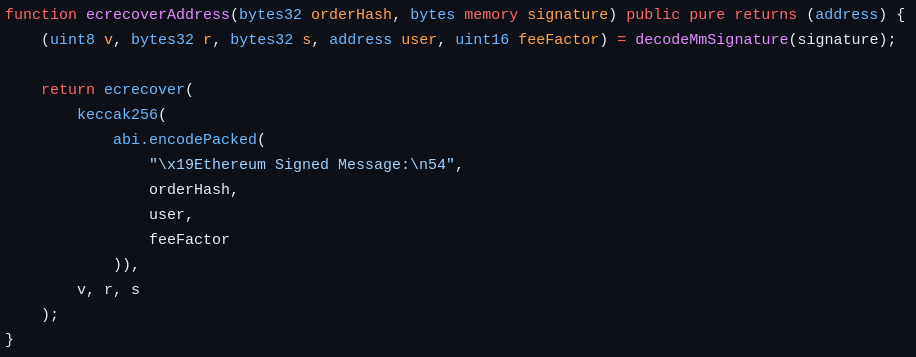
\includegraphics[width=0.89 \linewidth]{ecrecover/ecrecover_function_personal}
        \caption{Ecrecover function personal sign implementation}
        \label{fig:ecrecover_personal}
    \end{figure}

    \subsubsection{Uniswap}

    The \textit{Uniswap} category is the one that includes the largest number of security mechanisms.
    The figure~\ref{fig:ecrecover_uniswap} points out the usage of \textit{domainSeparator} but also \textit{nonce} and \textit{deadline}.

    This figure~\ref{fig:ecrecover_uniswap} also reveals the correct usage of \textit{nonce}.
    Indeed, they increase the value after the validation of the transaction preventing this way from \glspl{replayattack}.

    \begin{figure}[H]
        \centering
        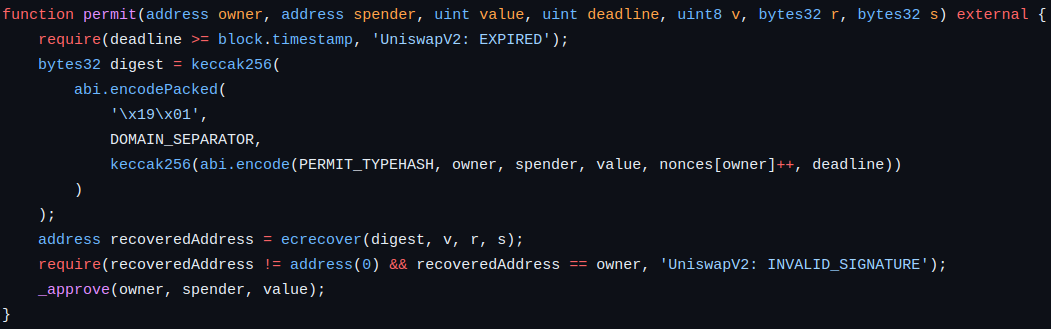
\includegraphics[width=0.9 \linewidth]{ecrecover/ecrecover_function_uniswap}
        \caption{Ecrecover function Uniswap implementation}
        \label{fig:ecrecover_uniswap}
    \end{figure}

    \subsubsection{OpenZeppelin}

    OpenZeppelin~\cite{openzeppelin} is a widely used framework that assists developers in building secure and reliable decentralized applications by offering pre-audited smart contracts, security best practices, and a supportive community.
    It has played a crucial role in advancing the security and usability of blockchain technology.

    $\\$

    Therefore, many \Glspl{dapp} implement the verification using OpenZeppelin.
    However, the figure~\ref{fig:ecrecover_openzep} presents a function without any verification tools mentioned above.
    Hence, even if OpenZeppelin provides all the tools necessary for a safe utilization, one can import and use directly this function.
    This could lead to a risk of vulnerability because the \Gls{dapp} could not implement the safeguards but still think, by using OpenZeppelin, that its application is secure.

    \begin{figure}[H]
        \centering
        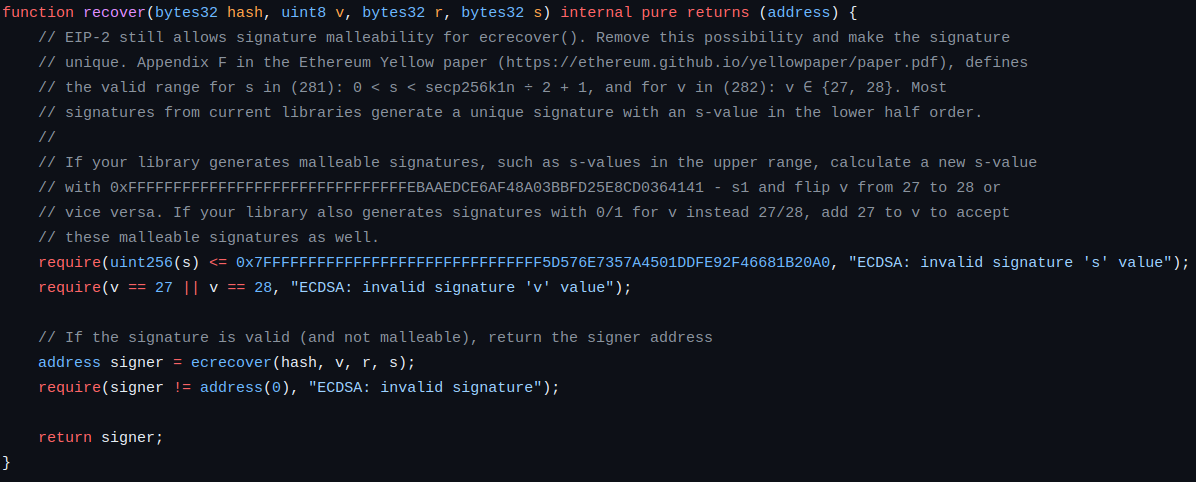
\includegraphics[width=0.9 \linewidth]{ecrecover/ecrecover_function_openzep}
        \caption{Ecrecover function OpenZeppelin implementation}
        \label{fig:ecrecover_openzep}
    \end{figure}

    \subsubsection{Compound}

    The last category is named \textit{Compound} after the most famous \Gls{dapp} that implements the signature verification this way.

    The main difference illustrated by the figure~\ref{fig:ecrecover_compound} is the absence of \textit{nonce} and \textit{deadline}.
    The \Glspl{dapp} in this category does not have every necessary tool to protect the user from malicious behavior.
    Even if it uses a \textit{domainSeparator}, the missing \textit{nonce} constitutes a vulnerability.

    \begin{figure}[H]
        \centering
        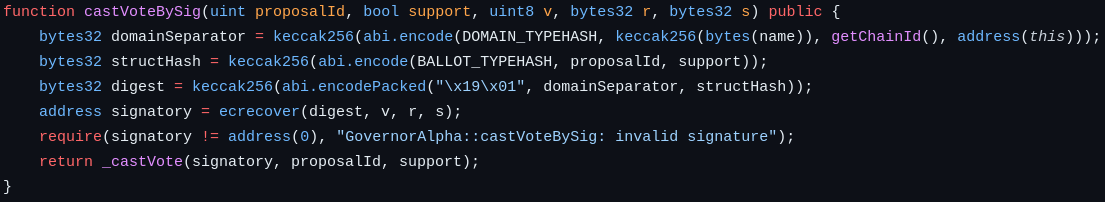
\includegraphics[width=0.9 \linewidth]{ecrecover/ecrecover_function_compound}
        \caption{Ecrecover function Compound implementation}
        \label{fig:ecrecover_compound}
    \end{figure}

    \subsubsection{Different}

    Finally, all the \Glspl{dapp} in this category have no similarity with the others.
    It does not impact the classification because, as the next section will show, this category does not contain a large number of \Glspl{dapp}.

    The figure~\ref{fig:ecrecover_different} points out the difference of this implementation from the others.
    Indeed, the hash given to the \textit{\gls{ecrecover}} function only contains \textit{commitLastBlock} and \textit{commit}.
    This allows the attacker to reproduce the signature verification on its malicious \Gls{dapp} leading to a potential loss of money or item.

    \begin{figure}[H]
        \centering
        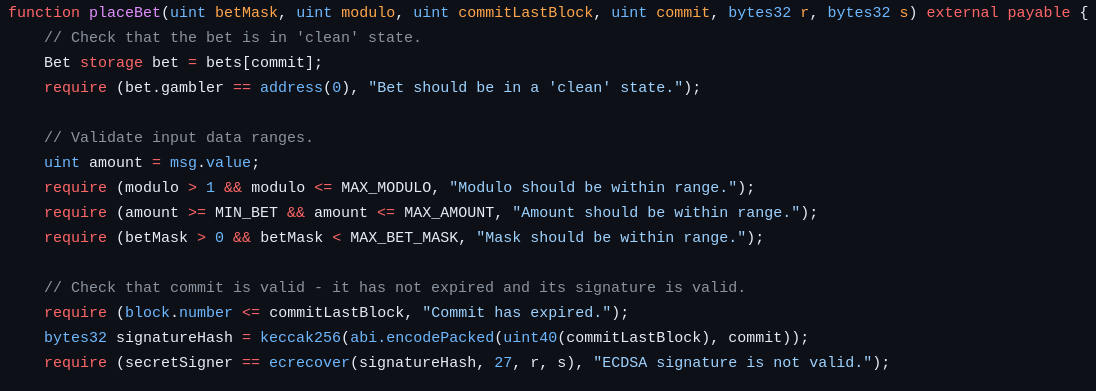
\includegraphics[width=0.9 \linewidth]{ecrecover/ecrecover_function_different}
        \caption{Ecrecover function different implementation}
        \label{fig:ecrecover_different}
    \end{figure}

    \clearpage

    \subsubsection{Repartition of DApps into this classification}

    The table~\ref{tab:comparison-categories} summarizes the main characteristics of the different categories exposed previously.

    \begin{table}[H]
        \begin{center}
            \begin{tabular}{|c||c|c|c|}
                \hline
                \textbf{Smart contract}   & \textbf{\textit{domainSeparator}} & \textbf{\textit{nonce}} & \textbf{\textit{deadline}}\\
                \hline
                \hline
                \textit{Uniswap}   & Yes & Yes & Yes             \\
                \hline
                \textit{OpenZeppelin}    & No in \textit{ecrecover} function    & No in \textit{ecrecover} function   & No in \textit{ecrecover} function   \\
                \hline
                \textit{Compound} &  Yes & No & No             \\
                \hline
            \end{tabular}
        \end{center}
        \caption{Summary of differences between \gls{smartcontract} categories}
        \label{tab:comparison-categories}
    \end{table}

    The figure~\ref{fig:repartition-ecrecover} represents the distribution of the different categories.

    \begin{figure}[H]
        \centering
        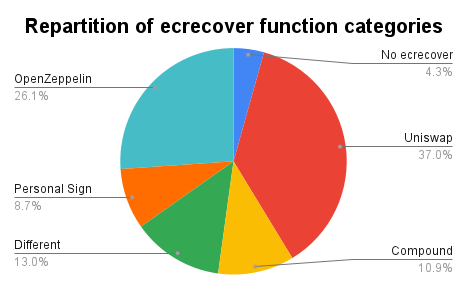
\includegraphics[width=0.69 \linewidth]{ecrecover/repartition_categories}
        \caption{Repartition of ecrecover function categories}
        \label{fig:repartition-ecrecover}
    \end{figure}

    It highlights that 37\% of the \Glspl{dapp} analyzed are \textit{Uniswap} which is the most secure category.
    However, 26\% of the \Glspl{dapp} can be unsafe with a wrong usage of \textit{OpenZeppelin} library.

    As mentioned before, the \textit{different}, \textit{personal sign} and no \textit{ecrecover}, which signifies that the \gls{smartcontract} just does not have any usage of \textit{ecrecover} function, represents only 26\% of the \Glspl{dapp}.

    Finally, about 11\% of the \Glspl{dapp} are part of the \textit{Compound} category which represents a vulnerability.
    This number is not insignificant and has to be reported.


    \section{Environmental and social impact}

    \subsection{Personal impact}

    As the project was almost only online, there was no commuting to work and no professional trip.
    This impact is therefore non-existent or negligible.

    I do not consider the first trip to go to the USA and the return to France because even without the project, those journeys would have been done.

    $\\$

    Most of my personal impact was the consumption of the equipment used for the project.
    The only piece of equipment used was my laptop.

    According to the website EcoInfo and their tool EcoDiag~\cite{ecodiag} my equipment has an impact corresponding to 101 kgCO2/year as the figure~\ref{fig:consumption} reckons.

    \begin{figure}[H]
        \centering
        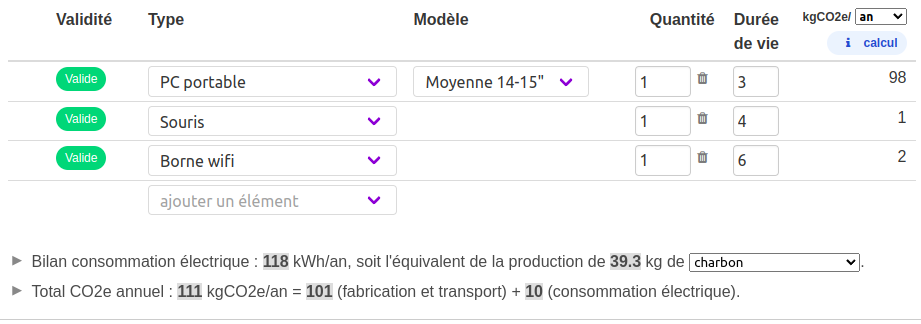
\includegraphics[width=0.9 \linewidth]{environmental_concern/electric_consumption}
        \caption{Environmental cost of equipment used during the project}
        \label{fig:consumption}
    \end{figure}

    Nevertheless, the electricity consumption impact cannot be used because the impact of electricity is different in the USA from France.

    In Illinois, electricity represents 0.855 pounds of CO2 emissions per kWh which means 0.388 kgCO2/kWh.
    The figure~\ref{fig:consumption} proposes annual consumption of 118 kW/year what means that the electricity consumption impact is 46 kgCO2/year.

    $\\$

    Therefore, the total cost is 147 kgCO2/year.
    As the project lasts around 220 days, the personal impact of the project is 89 kgCO2.

    It can be noticed that electric consumption plays a larger role in the impact in the USA rather than in France.

    \clearpage

    \subsection{Global impact}

    \subsubsection{Environmental impact}

    The energy consumption associated with some blockchain networks has raised concerns due to its environmental impact.
    Energy usage in blockchain technology is primarily attributed to the computational processes required for consensus mechanisms, transaction validation, and maintenance of the distributed ledger.

    However, the project analyzes blockchain technology but does not run these technologies.
    Therefore, energy consumption of \Glspl{dapp} are not linked with the project.
    Even if a \Gls{dapp} has been created for the project, it was running locally, and its impact has already been discussed in the personal analysis.
    The calls made to MetaMask represent a negligible environmental impact.

    $\\$

    The location of the team is a consideration that can be made.
    As we saw previously, between France and the USA, electricity represents a very different number of emissions.

    The team was located in Illinois, and it can be interesting to look for the difference between this state electricity impact and the US average one.

    The Illinois net electricity generation by source is 7\% natural gas, 30\% coal-fired, 54\% nuclear (most in the nation) and 10\% renewables, according to Illinois Environmental Council~\cite{iec}, a governmental institution.
    However, in the United States, according to the U.S. Energy Information Administration~\cite{eia}, the net electricity generation by source is 39.8\% natural gas, 19.6\% coal-fired, 18.2\% nuclear and 21.5\% renewables.
    This makes the US average electricity source emissions of 0.371 kgCO2/kWh whereas it is a bit higher in Illinois with 0.388 kgCO2/kWh.

    $\\$

    Enhancing security may sometimes mean increasing the consumption of applications.
    Indeed, if there is a need to make more verification, the scripts will run longer and therefore consume more energy.

    $\\$

    In the context of this project, we noticed that \textit{personal\_sign} was less efficient than \textit{eth\_signTypedData}.
    However, the analysis has highlighted that many \Glspl{dapp}, even in the most popular ones, uses \textit{personal\_sign} over its more efficient alternative.
    As those \Glspl{dapp} can be the source of huge traffic, even a slight improvement of performance can lead to massive saves of energy.

    $\\$

    For instance, OpenSea uses this method and has around 10,000 active users per day.
    Therefore, thanks to the work done on this project some users could prefer use applications that does not uses the \textit{personal\_sign} method.

    However, the beneficial impact induced by the project is not quantifiable but seems to be negligible.

    \clearpage

    As the project has no tangible application in industry, its environmental impact is very low.
    The analysis has developed tools, but these are not designed for a massive usage.
    Furthermore, the equipment required by the project was only composed of a computer and its impact has been calculated on the previous section.

    Finally, as the team was composed by four people, the carbon footprint of the project is around 400 kgCO2.
    This impact represents the carbon footprint of a French person during 13 days.

    \subsubsection{Societal impact}

    By providing users with information about the security levels of \Glspl{dapp}, the project can enhance user confidence in using blockchain applications.
    Users who are aware of the potential vulnerabilities and risks can make more informed decisions, leading to a safer and more trusted environment for blockchain adoption.

    The focus on vulnerabilities also educates users about the potential security risks associated with \Glspl{dapp}.
    This increased awareness can extend beyond the tools developed, promoting a culture of cybersecurity consciousness among blockchain users and developers.

    As developers become more aware of the vulnerabilities highlighted by the project, they may encourage adopting better security practices during development.
    This could lead to the overall improvement of security, reducing the prevalence of vulnerabilities.

    $\\$

    A more secure \Gls{dapp} environment can mitigate the risk of exploitation, theft, and unauthorized access.
    This can lead to fewer incidents of financial loss suffered by users and businesses.
    Indeed, exploitation and theft often target end-users who might unknowingly interact with compromised \Glspl{dapp}.
    By providing users with information about the security status of \Glspl{dapp}, the project empowers them to make informed decisions.
    Users can avoid using \Glspl{dapp} with known vulnerabilities, minimizing their exposure to potential threats.

    $\\$

    About the privacy policy, all the data collected by the tools was publicly accessible and was not sensible.
    Moreover, the tools only collect data about applications or websites that do not contain personal data.

    $\\$

    Finally, the analysis plays a crucial role in reducing exploitation within the blockchain ecosystem by identifying vulnerabilities, promoting early detection and remediation, and enhancing user awareness and protection.
    By addressing these issues, the project contributes to a more secure and trustworthy environment for blockchain applications and transactions.


    \subsection{Illinois Institute of Technology policy}
    
    \subsubsection{Sustainability Integration in Curriculum}

    As Illinois Institute of Technology is a university, the most obvious positive action that it can lead is educating people about environment and social concerns.

    The incorporation of sustainability principles, concepts, and practices across various academic disciplines and courses.
    The goal is to educate students about the interconnectedness of environmental, social, and economic systems, and to equip them with the knowledge and skills needed to address complex global challenges in a sustainable manner.

    $\\$

    However, this action can suffer from potential negative aspects.
    Not all educators may be well-versed in sustainability concepts or just may not want to integrate these issues into their classes.
    This could result in inconsistent or insufficient coverage of sustainability topics in certain courses.

    If not properly managed, adding sustainability content to existing courses might result in information overload for students, potentially diluting the overall learning experience.
    Students could question the relevance of the learning, and even doubt about the necessity to take actions.

    $\\$

    Integrating sustainability into the curriculum is a significant step towards fostering environmentally and socially responsible citizens.
    While there are potential challenges, such as faculty adherence and curriculum management, the positive aspects outweigh the negatives.
    Proper training for educators and ongoing assessment can help ensure that sustainability integration effectively equips students with the knowledge and mindset needed to address the complex challenges of our world.

    \subsubsection{Energy-efficient practices}

    One of the main challenges to address is the energy consumption.
    This action involves adopting technologies, behaviors, and strategies that aim to minimize energy consumption while maintaining or improving functionality.
    These practices are crucial for reducing the environmental impact of energy production, conserving natural resources, and mitigating climate change.

    $\\$

    Energy-efficient practices directly contribute to lowering greenhouse gas emissions.
    By consuming less energy, institutions like the Illinois Institute of Technology can help decrease their carbon footprint and combat climate change.
    They announce that they develop energy performance contracts on campus to reduce wasted energy through higher efficiency equipment, more building controls.
    They want to shift loads using geothermal heating and cooling, using daylight and passive strategies.

    \clearpage

    Nonetheless, no document with clear objectives in duration and in energy consumption reduction could have been found.
    Moreover, natural gas is used as a source of energy for heating buildings and generating hot water.
    Although natural gas is relatively clean burning fossil fuel, it is not a renewable resource leading.

    $\\$

    However, as many places in the United States, every building is equipped with air conditioning.
    IIT could increase the temperature, which is set really low in my experience, to significantly reduce the energy consumption.
    It can use air conditioning less often and only in necessary places.

    \section{Conclusion}

    \subsection{Project conclusion}

    The analysis of the usage of signing methods has revealed that a lot of \Glspl{dapp} are subjects to the vulnerability of \textit{eth\_sign}.
    Furthermore, even if the usage of this unsafe method occurs more often in less famous \Glspl{dapp}, several famous ones are vulnerable because of the usage of this method.

    $\\$

    Nonetheless, using a safer method such as \textit{eth\_signTypedData} does not prevent from having vulnerabilities.
    Indeed, the \textit{domainSeparator} field, normally used to prevent someone from using a signature in another \Gls{dapp}, is not verified correctly by MetaMask.
    This can induce developers to not include every security field introduced by EIP712.

    $\\$

    Moreover, some \Glspl{dapp} implements the signature verification without using a mechanism that makes the signature unique.
    The \textit{Compound} category and its non-negligible number of \Glspl{dapp} has shown an unsecure behavior in several applications.

    Finally, the OpenZeppelin category also draws attention because of its potential lack of security when developers does not use the library the right way.x


    \subsection{Future work}

    Collecting even more \Glspl{dapp} is a way to extend the analysis.
    One way would be to overpass the limitation of the GitHub \Gls{api}.
    This may be possible by selecting the results from a date to another date.
    Thereby, there would be less than a thousand results after a call to the \Gls{api}.
    Indeed, changing the date corresponds to querying another time the \Gls{api}.
    The challenge is to find the best range of date to not multiply the calls and not to have more than a thousand results.

   $\\$

    Furthermore, several \Glspl{dapp} seems to be particularly vulnerable.
    For instance, Demex and Accross protocol have drawn attention.
    The first one has a fixed string as \textit{verifyingContract} inside its \textit{domainSeparator} instead of a dynamic value corresponding to the real contract.
    The second one does not include any \textit{verifyingContract} on the \textit{domainSeparator}.
    These two examples shine a light on the need of verifying the value of every field of \textit{domainSeparator}.

    \clearpage

    \subsection{Personal conclusion}

    This project has been an important development for my academic and research growth.
    It has given me the tools to delve further into blockchain technology and cybersecurity.

    $\\$

    Moreover, the discovery of blockchain and \Glspl{dapp} operation has provided me with a profound appreciation for the decentralized spirit that supports these innovations.
    Witnessing the power of cryptographic principles and the benefits of decentralization has strengthened my perspective on the possibilities that blockchain technology can offer to various industries.

    $\\$

    As I reflect on this project, I realize it has ignited a curiosity to continue exploring and learning.
    The challenges I have faced and the knowledge I have acquired have deepened my understanding and passion for this field.
    I look forward to pursuing further studies in a PhD program, drawing from both the technical skills and the research experience I've gained here.

    % Bibtex
    \bibliographystyle{plainurl}
    \bibliography{main}
    
    \clearpage

    \begin{appendices}
        \section{Bash script to find signing methods}
        \label{sec:find-signing-methods-script}

        \lstinputlisting[language=bash]{../resources/appendix/finderGithub.sh}

        \section{Bash script that automate the analysis of signing methods}
        \label{sec:combine-all-scripts}

        \lstinputlisting[language=bash]{../resources/appendix/findInGithubSearch.sh}
    \end{appendices}





\end{document}
